\chapter{Materials and Methods}\label{chap:methods}
The challenges in genomic analysis of viral material using NGS raw read data are the major motivation for this thesis. Ready-to-use pipelines that can be executed without deeper biological or bioinformatical knowledge specifically designed for the viral genomes of avian influenza, pox and foot-and-mouth disease are presented below. They run on the Galaxy platform and show that for development of the pipelines, large parts of existing viral genomic analysis pipelines as such for SARS-CoV-2 can be reused and adapted.

\section{Galaxy Platform}\label{sec:galaxy}
Galaxy is a web-based scientific platform that has become a major player in many fields of life sciences and bioinformatics. Founded in 2007 it has provided an emerging amount of resources and tools to empower scientists and researchers to work with biomedical datasets. The platform is free to use and collaborative, making it one of the biggest of its kind. Resources on Galaxy cover genomics, metagenomics, transcriptomics, proteomics, drug discovery and non-biology fields like natural language processing and social sciences.

Galaxy's primary objective is to make analyses more accessible, reproducible, and easier to communicate among researchers. The platform's distinctive and success is attributed to four core elements: a very active community, a public server for analyses, an open-source software ecosystem, and the Galaxy ToolShed. The community adheres to the FAIR practises (Findable, Accessible, Interoperable and Reusable)~\cite{10.1093/nar/gkac247}.

The Galaxy community is thriving, with over 124,000 users who also contribute to subcommunities. The public server for analyses provides access to public datasets and workflows. The open-source software ecosystem ensures automated setup and deployment of all tools and services, making it simple for beginners and professionals to use. The Galaxy ToolShed is a server dedicated to hosting, sharing, and installing tools used on the platform. A Galaxy tool is the abstraction layer that makes external software usable from within Galaxy with a frontend, i.e. lets users use the program with all its parameters and inputs from within Galaxy. \\ 
Galaxy workflows are a key feature that allow the user to stack tools in a chain and to configure them so that the workflow user only has to upload his or her data for the input fields. The automation of tools in a chain is used for modular, longer analyses that are executed repeatedly. \\
Workflows that are available on and accepted by the Intergalactic Workflow Commission (IWC; \url{https://github.com/galaxyproject/iwc}) are conform with the community's best practise standards and tested on the latest Galaxy release. Dockstore and WorkflowHub automatically publish the \acs{IWC} workflows and guarantee the availability in a Docker-based environment on Dockstore~\cite{o2017dockstore} and on the workflow collaboratory WorkflowHub~\cite{goble2021implementing}.

Important contributions of Galaxy, as stated by the Galaxy Community (2022), include Vertebrate Genome Project assembly workflows and collaborations about \ac{SARS-CoV-2} research. Another toolkit leveraged in Galaxy is Galaxy-ML, a set of tools that form a suite for analyses based on machine learning. With growing publicity, more topics are covered by and moved to Galaxy. It has contributed to over 5,700 scientific publications and has many tutorials available for researchers to use. Training material and ready-to-use workflows facilitate professionals and beginners in the field to use Galaxy for their research purposes. \\
The Galaxy platform is continuously enhanced, and it still attracts around 2,000 new users every month, indicating its quality and significance. The team and infrastructure of Galaxy initially come from the Nekrutenko lab in the Center for Comparative Genomics and Bioinformatics at Penn State, the Taylor lab at Johns Hopkins University, and the Goecks Lab at Oregon Health \& Science University. All of these organisations have contributed significantly to the success of Galaxy. There are 138 public servers available worldwide as of 2023, while the most prominent general-purpose server instances are hosted by teams at University of Freiburg, Germany (for \href{https://usegalaxy.eu/}{UseGalaxy.eu}), Texas Advanced Computing Center (for \href{https://usegalaxy.org/}{UseGalaxy.org}) and Genomics Virtual Laboratory, formerly at the University of Queensland (for \href{https://usegalaxy.org.au/}{UseGalaxy.org.au}). These main public servers are synchronised in their tools and set of reference tools~\cite{10.1093/nar/gkac247}.

\section{Reusing Components of Existing SARS-CoV-2 Pipelines}
\todoit
\ac{SARS-CoV-2} Pipeline as Baseline. -> ampliconic iVar-based Workflow for Illumina reads.
(annotated) variants are of interest \\

Plus Variant Calling and genome annotation; \\
Plus phylogenetic ranking ``to assign a \ac{SARS-CoV-2} genome sequence the most likely lineage based on a chosen nomenclature system'' (Pangolin)

\subsubsection{Requirements for Poxvirus Workflow}
As explained in~\secref{sec:2-pox}, the genome of most poxviruses is bound by identical sequences located at the termini of the genome. It is shown that the size of such differs for some poxviruses, such as rabbitpox and vaccinia virus, while monkeypox, cowpox and capripoxviruses have shorter \acp{ITR}~\cite{wittek1978inverted}. For a whole-genome reconstruction from \ac{HTS}-generated reads, alignment algorithms look for the unambiguous location of a read. Since this is impossible for repeated sequences neither for reference-based mapping approaches nor \textit{de novo} assembly, a new approach has to be used that splits the sequencing reads into two parts, separating the identical sequences and running alignment algorithms for each of the splits. To build the full-length genome, the alignments need to be ``glued'' together. This approach requires the reads to be sequenced in two pools with two libraries. A similar protocol has been described by Mathijs et al. and the ARTIC network for SARS-CoV-2 data~\cite{mathijs2022robust, tyson2020improvements}. \\
Other requirements for a reference-based surveillance of the genomics of poxviruses include the availability of the primer scheme that was used for amplicon-based sequencing with an Illumina sequencer. The \ac{BED} file containing the primers, their positions and the pool identifier is essential for the correct linking of the alignments when splitting the pipeline into two parts and merging it back together.

\subsubsection{Requirements for AIV Workflow}
The main objectives of surveillance of \ac{AIV} on the genetic level are to get phylogenetic insights and to check for new variants that could occur in the \ac{HA} and \ac{NA} proteins as a consequence of reassortment. \\
A pipeline for an avian influenza virus sample that should build a consensus sequence in order to check for mutations needs a reference sequence that it can align the sequence to. A main caveat of many existing pipelines is the user's choice of reference sequence, since it is an arbitrary choice and there are many different reference sequences to choose from. Therefore, a dynamic approach that is sensitive enough for the segmented structure of the \ac{AIV} genome is needed. The diversity of \ac{HA} and \ac{NA} segments' sequences is significant enough to make it challenging to map sequenced reads to a single, full-length influenza A reference sequence. Although this approach may be effective for the other six segments, the mapping software would frequently be unable to locate sufficient plausible matches for sequenced reads of \ac{HA} and \ac{NA} origin to continue with the analysis. By using a splitting approach that finds the best reference sequence from a database, the expensive assembly step is avoided and mapping can be conducted. \\
Compared to analyses with similarly large genomes such as \ac{SARS-CoV-2} and due to the segmented structure of the \ac{AIV} genome, duplicates among the mapped reads of the \ac{AIV} sample should not be dismissed but kept for maintaining a reasonable high coverage for the further analyses. 

\subsubsection{Requirements for FMDV Workflow}
\todoit
multisample, VAPOR, mapping (de novo assembly for control?)

\section{Workflow Development}
Galaxy workflows for the specific viruses that account for the genomic structure of each virus are described below.

\subsection{Poxvirus Illumina Amplicon Workflow}\label{sec:pox-wf}
The proposed Galaxy workflow for poxvirus samples that were Illumina-sequenced with a tiling amplicon approach is available on the WorkflowHub, Dockstore and Galaxy EU~\todo{links}. It aims at constructing the full genome from Illumina-sequenced reads and providing alignment files, the constructed consensus sequence and intermediate results and reports that give insights into reads, mapping quality and mapping coverage. An overview of these outputs and the respective datatypes is provided in Supplementary~\tabref{tab:pox-outputs}. \\
To account for the repeated \acp{ITR} at the ends of the poxvirus genome, the workflow is based on a tiled amplicon approach. During the first steps, the reads of the two pools from each genome half are processed individually as half genomes. Input data for the workflow are the reads from pool1 and pool2, sourced from the sequencing with two libraries; the used primer scheme in \ac{BED} file format that contains an indicator for pool1 or pool2 in the \textit{SCORE} column, and a reference sequence that is used for mapping. 

\begin{figure}[ht!]
	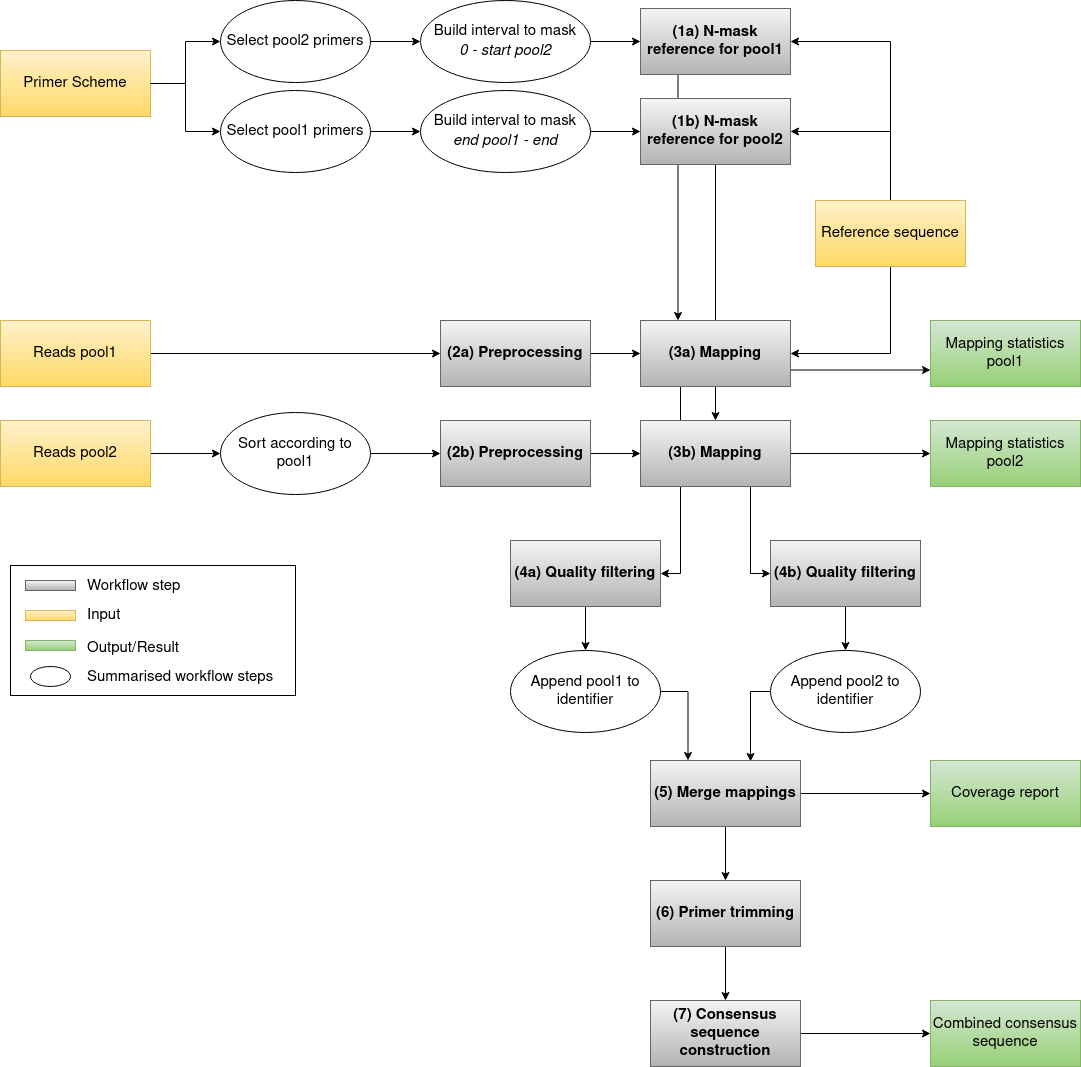
\includegraphics[width=1\textwidth]{media/3-pox.png}
	\caption{Simplified poxvirus genomic analysis workflow for ampliconic Illumina-sequenced data.}
	\label{fig:3-pox-wf}
\end{figure}

As a first step, (1) the provided reference sequence is prepared for the mapping of the two pools. Hence, the primer scheme is needed to compose the exact intervals so that the remaining bases are N-masked. For mapping pool1 against the reference, the second half is N-masked and therefore the interval for the remaining bases is built, while the second half of the reference sequence is N-masked. The masking starts at the minimal start position of the first primer of pool2. Accordingly for the mapping of pool2, the interval of the remaining bases is constructed by taking the maximal end position of the pool1 primers and the full length of the reference sequence so that the masking of the first half can be conducted. The construction of the text parameter in the correct input format is done by multiple Galaxy-specific text-processing tools and can be looked up in the Supplementary~\tabref{tab:aiv-tools-steps}. \\
The workflow is designed to process multiple samples in one run, thus the samples of both pools are sorted by the order of how they are listed in pool1. Before mapping, (2) the reads of both pools are preprocessed with \texttt{fastp} to automatically trim Illumina-specific PolyG tails of the reads. The following (3) mapping step with \texttt{BWA-MEM} takes the corresponding masked reference sequence for each genome-half. A statistics report for each alignment is generated using \texttt{Samtools stats} to check for the quality of the mapping. The alignments are (4) filtered for quality with \texttt{Samtools view} to keep reads with a minimum length of 20 and only properly paired and mapped reads, and the pool identifiers (\textit{pool1/pool2}) are prepended to the sample names so that using external software to check variants, the pool and sample identification is maintained. The next step (5) joins the two alignments while retaining the identifiers for each sample and pool. For the mapping of the whole-genome, a coverage report is generated with \texttt{QualiMap BamQC} so that the \acp{ITR} and the part where the mappings are merged can be inspected. (6) Primer-trimming with \texttt{iVar trim} removes the loose primer ends and cleans the alignment for the consensus sequence construction. The (7) consensus sequence is called with \texttt{iVar consensus} for which the user can use either provided default settings (minimum quality score to count base: 20, minimum allele frequency threshold to call SNV: 0.7, minimum allele frequence to call indel: 0.8) or enter their own values before starting the workflow. The workflow with a complete list of the 47 steps, used tools, parameters and their versions as well as outputs and connections between the tools is provided in Supplementary~\tabref{tab:pox-tools-steps}. 

\subsection{AIV Illumina Workflow}\label{sec:aiv-wf}
% explain SNPs
We propose a fully automated pipeline for the analysis of Illumina-sequenced paired-end reads from avian influenza samples. The workflow is integrated in the Galaxy platform and available via \todo{link}. It is designed to take one input sample at a time and besides a summarising results report, the outputs of the analysis steps can be used for further research based on the user's interest. The workflow is outlined in~\figref{fig:3-aiv-wf}, where the nine main steps of the workflow are visualised. The full workflow of 48 steps with the tools, tool version and parameters can be found in Supplementary~\tabref{tab:aiv-tools-steps}. \\
One novelty of the workflow is the consideration of the different segments of the influenza virus genome. After uploading paired-end reads and a reference sequence database, which is available online too \todo{link}, the workflow builds a hybrid reference from the given database for each of the segments of the genome. The reference sequence database consists of eight FASTA files, one per segment, containing numerous full-length sequences for a given segment. The provided database file consists of 56 sequences for each segment. If a user decides to upload their own references, it is important to follow the sequence identifier pattern so that the extraction of sequence identifiers works: >\textit{segment\_name$\mid$influenza\_strain$\mid$subtype$\mid$accession\_number}. For example, one entry's identifier is >\textit{PB1$\mid$A/duck/Manitoba/1953$\mid$A/H10N7$\mid$KF435047.1} followed by the sequence in the next line. 

\begin{figure}[ht!]
	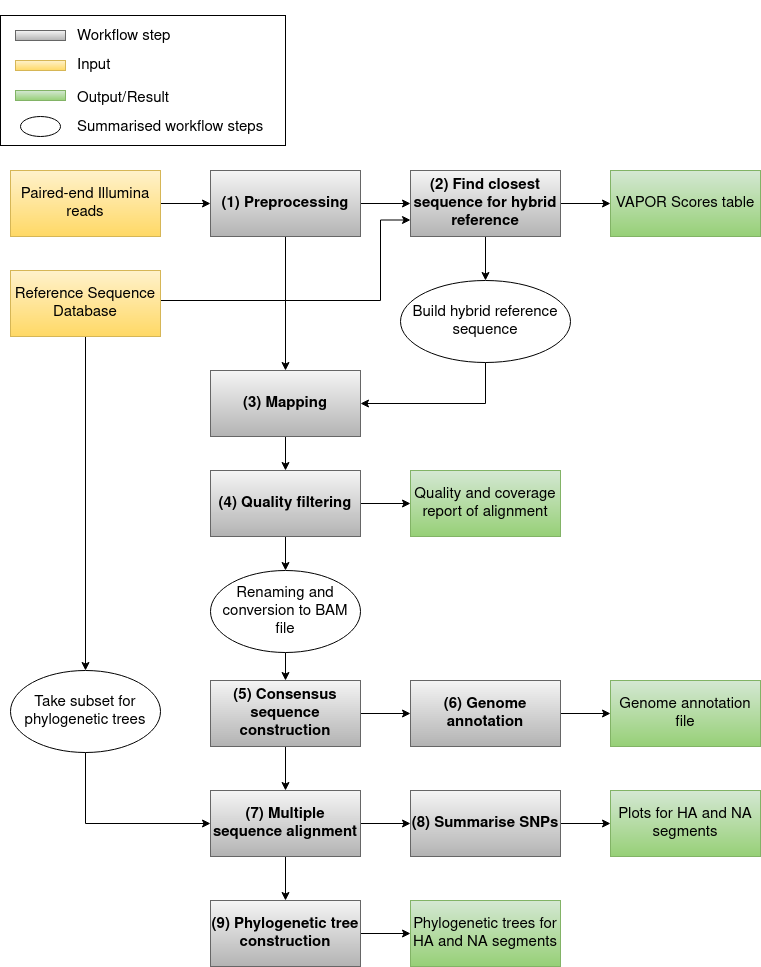
\includegraphics[width=1\textwidth]{media/3-aiv.png}
	\caption{Simplified \ac{AIV} genomic analysis workflow for Illumina-sequenced data.}
	\label{fig:3-aiv-wf}
\end{figure}

After (1) preprocessing of the reads with \texttt{fastp} to dismiss reads shorter than 30 basepairs and automatic trimming PolyG tails of the Illumina reads, the database of reference sequences is used to (2) find the closest possible reference for each of the segments. The tool \texttt{VAPOR} outputs a table with a scoring based on the graph construction, and should not be confused with the identity of the sequence compared to the reference. As \texttt{VAPOR} is running once per segment but has independent inputs, this step is executed in parallel. \texttt{VAPOR} is a graph-based classifier that maps k-mers to a weighted De Bruijn graph~\cite{southgate2020influenza}. Its benchmarking shows that it runs significantly faster than \ac{BLAST} and default configuration leads to reasonable matches similar to Mash, as long as the given sample is not very different from or novel to the provided sequences in the reference database. \\
Using the highest scoring sequences from the eight \texttt{VAPOR} runs, a hybrid reference sequence is built. To control the statistics of the graph and adapt the configuration, a table with the highest \texttt{VAPOR} scores of each run is generated. \\
The hybrid reference sequence is composed of the eight segments and is used for the third step of the pipeline, (3) mapping with \texttt{BWA-MEM}. The segment names in the hybrid reference genome are truncated and shortened to just the segment identifier. Mapping of the preprocessed reads against the prepared hybrid reference is run with default parameters of \texttt{BWA-MEM}. The \ac{BWA-MEM} algorithm aligns 70-1000 basepairs long reads by seeding alignments with maximal exact matches, and extending the seeds using the affine-gap Smith-Waterman algorithm~\cite{li2013aligning}. After mapping, the resulting \ac{BAM} dataset is (4) quality filtered using \texttt{Samtools view}. Reads with a minimum quality of 20 and those that are paired and mapped in a proper pair are kept. The alignment and quality results as well as coverage statistics for each segment are reported using \texttt{QualiMap BamQC}. \\
The subsequent steps before generating the consensus sequence of the sample prepare the \ac{BAM} file and deconstruct the mapped reads into a collection of eight datasets and relabel the elements, so that (5) \texttt{iVar consensus} can perform consensus sequence construction in parallel. 
Per-segment consensus construction is run with a minimum quality score threshold of 20, minimum frequency threshold of 0.7, minimum depth to call consensus of 10, does not exclude regions with smaller depth than the minimum threshold and uses N instead of - for regions with less than the minimum coverage. These settings accept any base as the consensus base for a genome position with a base calling quality of 20 or higher in order to avoid false bases that come from sequencing errors. If there is no consensus base to be found with the above thresholds, an N is inserted instead. \\
The next step using the consensus sequence is (6) generating genome annotation files with \texttt{Prokka}. As the input sample is a viral genome, the \textit{Kingdom} parameter is set to \textit{Viruses}. With this file, open reading frames can be predicted using web-tools and further downstream analyses can be started. \\
To place the consensus sequence of the avian influenza segments in a set of samples from the reference sequences, (7) a multiple sequence alignment for a user-specified number of sequences (i.e. determines the size of the resulting phylogenetic trees) is conducted with \texttt{MAFFT} (Multiple Alignment using Fast Fourier Transform) and the consensus sequence is added using \texttt{MAFFT add}. The multiple sequence alignment is also used for (8) a visualisation of SNPs, produced with the \texttt{snipit} tool. \\
As a final step, (9) phylogenetic trees for the \ac{HA} and \ac{NA} segments are built using \texttt{IQ-Tree}. The taxonomy of the sample segments visualised in the phylogenetic trees give insight into spatial and temporal spread of the genome. The consensus sequence from the input sample is assigned to the most likely lineage~\cite{minh2020iq}. \\
The presented workflow avoids the computationally expensive \textit{de novo} assembly, instead uses a mapping approach with a dynamically composed reference sequence of close sequences for each of the eight influenza segmets. This accounts for a high quality mapping and is evaluated in~\chapref{sec:4-aiv}. To control and look up intermediate outputs, quality reports are emitted during the workflow process and after finishing, can be downloaded as a \ac{PDF} for each workflow run. \\
Due to a variety of possible downstream analyses that can be of the user's interest, the pipeline provides intermediate results of the individual steps so that they can be used with other tools. An overview of these outputs with their datatype is provided in~\tabref{tab:aiv-outputs}. Possible downstream analyses are discussed in~\chapref{chap:discussion}.

% Kraken2 vs. VAPOR; 
% Efficiency: LoFreq vs. iVar consensus; both consensus identification methods using the same site-specific depth threshold

\subsection{FMDV Illumina Amplicon Workflow}\label{sec:fmdv-wf}
\todoit

multisample, VAPOR, mapping (de novo assembly for control?)

\begin{figure}[ht!]
	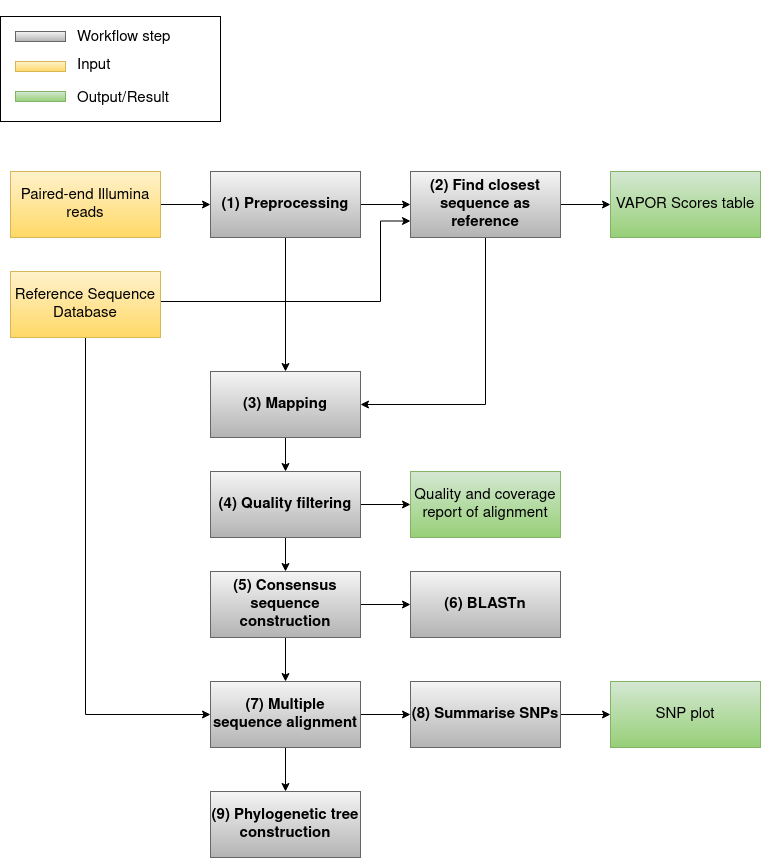
\includegraphics[width=1\textwidth]{media/3-fmdv.png}
	\caption{Simplified \ac{FMDV} genomic analysis workflow for ampliconic Illumina-sequenced data.}
	\label{fig:3-fmdv-wf}
\end{figure}
